\documentclass[autodetect-engine,dvi=dvipdfmx,ja=standard,
               a4j,11pt]{bxjsarticle}

\RequirePackage{geometry}
\geometry{reset,paperwidth=210truemm,paperheight=297truemm}
\geometry{hmargin=.75truein,top=20truemm,bottom=25truemm,footskip=10truemm,headheight=0mm}
%\geometry{showframe} % 本文の"枠"を確認したければ,コメントアウト
\usepackage{graphicx}
\usepackage{subcaption}
\usepackage{fancyvrb}
\usepackage{spverbatim}
\usepackage{amsmath}
\renewcommand{\theFancyVerbLine}{\texttt{\footnotesize{\arabic{FancyVerbLine}:}}}

\title{画像処理実験 第3回}
\author{学生番号: 09B23523\\
        大野颯也 (OHNO, Soya)}
\date{\number\year 年\number\month 月\number\day 日}

%%======== 本文 ====================================================%%
\begin{document}
\maketitle
% 目次つきの表紙ページにする場合はコメントを外す
%{\footnotesize \tableofcontents \newpage}


%--------------------------------------------------------------------%
%\begin{Verbatim}[numbers=left, xleftmargin=10mm, numbersep=6pt,
%                    fontsize=\small, baselinestretch=0.8]
%def main():
%  s=[ord('A'), ord('B'), ord('C')]
%  print(s)
%  print(bytes(s).decode())
%\end{Verbatim}

%--------------------------------------------------------------------%
%\section{数式: 行列,ベクトル}

%\newcommand\bA{\mbox{\boldmath$A$}}
%\newcommand\bb{\mbox{\boldmath$b$}}
%太字$\bA$を使えるように定義した.
%$\bA^{-1}\bb$等,使う文字を newcommand で定義して使う.

% \boldsymbol{A} は使えない


%--------------------------------------------------------------------%




%--------------------------------------------------------------------%
\section{第3回} \label{sec:abstract}
\subsection{課題3.1}
\subsubsection{関数,bの作成}
特徴座標 w が,
\[
w =
\begin{pmatrix}
x_0 & y_0 & u_0 & v_0 \\
x_1 & y_1 & u_1 & v_1 \\
x_2 & y_2 & u_2 & v_2 \\
x_3 & y_3 & u_3 & v_3 \\
\end{pmatrix}
\]

であるので,行列A,bは以下のようになる.
\[
w =
\begin{pmatrix}
x_0 & y_0 & 1 & 0 & 0 & 0 & -u_0 x_0 & -u_0 y_0 \\
0 & 0 & 0 & x_0 & y_0 & 1 & -u_0 x_0 & -u_0 y_0 \\
x_1 & y_1 & 1 & 0 & 0 & 0 & -u_1 x_1 & -u_1 y_1 \\
0 & 0 & 0 & x_1 & y_1 & 1 & -v_1 x_1 & -v_1 y_1 \\
x_2 & y_2 & 1 & 0 & 0 & 0 & -u_2 x_2 & -u_2 y_2 \\
0 & 0 & 0 & x_2 & y_2 & 1 & -v_2 x_2 & -v_2 y_2 \\
x_3 & y_3 & 1 & 0 & 0 & 0 & -u_3 x_3 & -u_3 y_3 \\
0 & 0 & 0 & x_3 & y_3 & 1 & -v_3 x_3 & -v_3 y_3 \\
\end{pmatrix}
\]
\[
b^\top =
\begin{pmatrix}
u_0 & v_0  & u_1 & v_1 & u_2 & v_2 & u_3 & v_3\\
\end{pmatrix}
\]

そして,以下がコードである.ここでは,後の課題で任意の個数の特徴点に合わせれるように,\verb|N=w.shape[0]| で作成する行列の行数も変更するようにしてある.

\begin{Verbatim}[numbers=left, xleftmargin=10mm, numbersep=6pt,
                    fontsize=\small, baselinestretch=0.8]
def makeAb(w):
  N=w.shape[0]
  A=np.zeros((N*2,8),'d')
  b=np.zeros(N*2,'d')
  i=np.arange(N)
  A[i*2+0,0]=w[i,0]
  A[i*2+0,1]=w[i,1]
  A[i*2+0,2]=1
  A[i*2+0,6]=-w[i,0]*w[i,2]
  A[i*2+0,7]=-w[i,1]*w[i,2]
  A[i*2+1,3]=w[i,0]
  A[i*2+1,4]=w[i,1]
  A[i*2+1,5]=1
  A[i*2+1,6]=-w[i,0]*w[i,3]
  A[i*2+1,7]=-w[i,1]*w[i,3]
  b[i*2    ]=w[i,2]
  b[i*2+1  ]=w[i,3]
  return A,b
\end{Verbatim}

実行した結果は以下のようになる.

\begin{Verbatim}[numbers=left, xleftmargin=10mm, numbersep=6pt,
                    fontsize=\small, baselinestretch=0.8]
[[256.00 218.00   1.00   0.00   0.00   0.00 -94976.00 -80878.00]
 [  0.00   0.00   0.00 256.00 218.00   1.00 -58880.00 -50140.00]
 [347.00 220.00   1.00   0.00   0.00   0.00 -160661.00 -101860.00]
 [  0.00   0.00   0.00 347.00 220.00   1.00 -79810.00 -50600.00]
 [263.00 367.00   1.00   0.00   0.00   0.00 -100729.00 -140561.00]
 [  0.00   0.00   0.00 263.00 367.00   1.00 -99677.00 -139093.00]
 [413.00 315.00   1.00   0.00   0.00   0.00 -218890.00 -166950.00]
 [  0.00   0.00   0.00 413.00 315.00   1.00 -135051.00 -103005.00]]
[371.00 230.00 463.00 230.00 383.00 379.00 530.00 327.00]
\end{Verbatim}

例と値が同じであるので,正しく動いている.




\subsection{課題3.2}
\subsubsection{calcHomography で計算した H を使った画像合成}
図\ref{fig:3.2_1.jpg}が H を使って生成した合成画像である.

\begin{figure}[h]
 \centering
 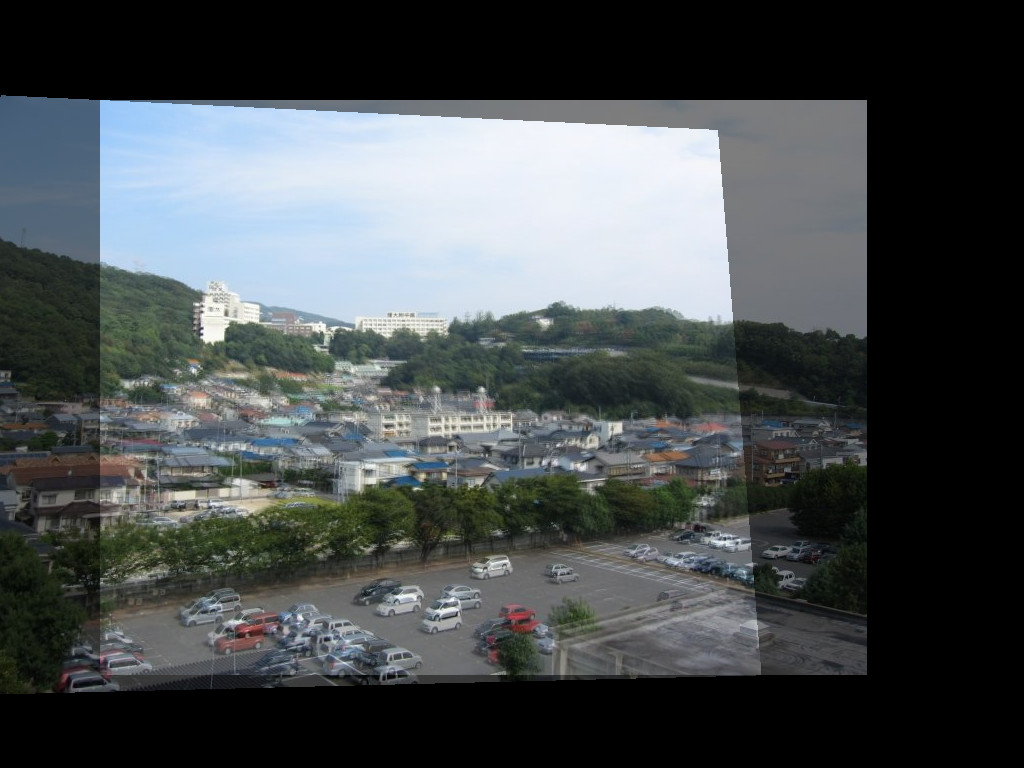
\includegraphics[scale=.3]{3.2_1.jpg}
 \caption{H を使った画像合成}
 \label{fig:3.2_1.jpg}
\end{figure}


\subsubsection{合成画像の品質の改善}
図\ref{fig:3-1.W-4.jpg}が特徴座標 w を変更して得られた合成画像である.

\begin{figure}[h]
 \centering
 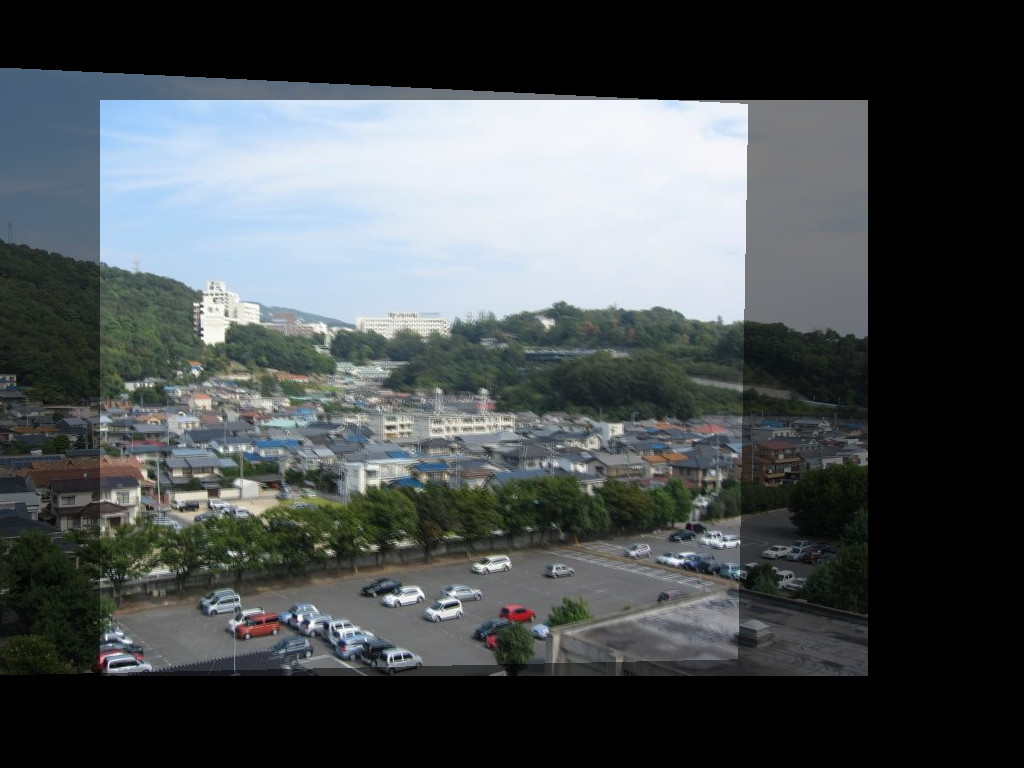
\includegraphics[scale=.3]{3-1.W-4.jpg}
 \caption{品質が改善された合成画像}
 \label{fig:3-1.W-4.jpg}
\end{figure}

\begin{figure}[h]
 \centering
 \begin{subfigure}[b]{0.45\textwidth}
   \centering
   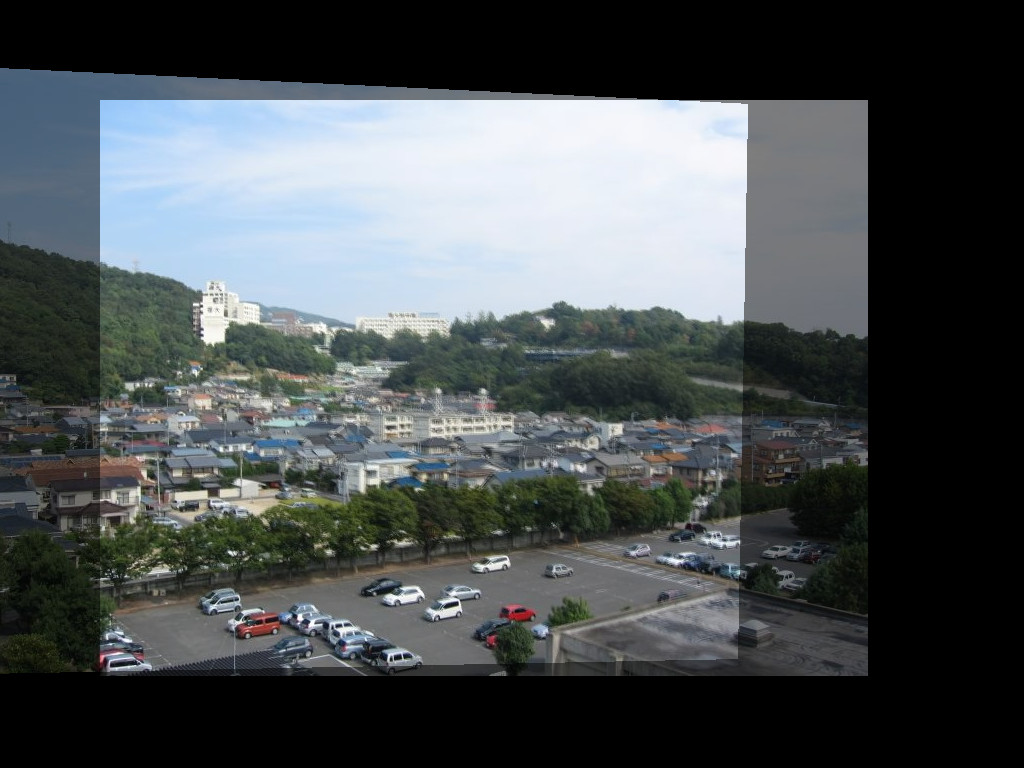
\includegraphics[scale=0.2]{3-1.W-8.jpg}
   \caption{特徴点8個の合成画像}
   \label{fig:3-1.W-8.jpg}
 \end{subfigure}
 \hspace{5mm}
 \begin{subfigure}[b]{0.45\textwidth}
   \centering
   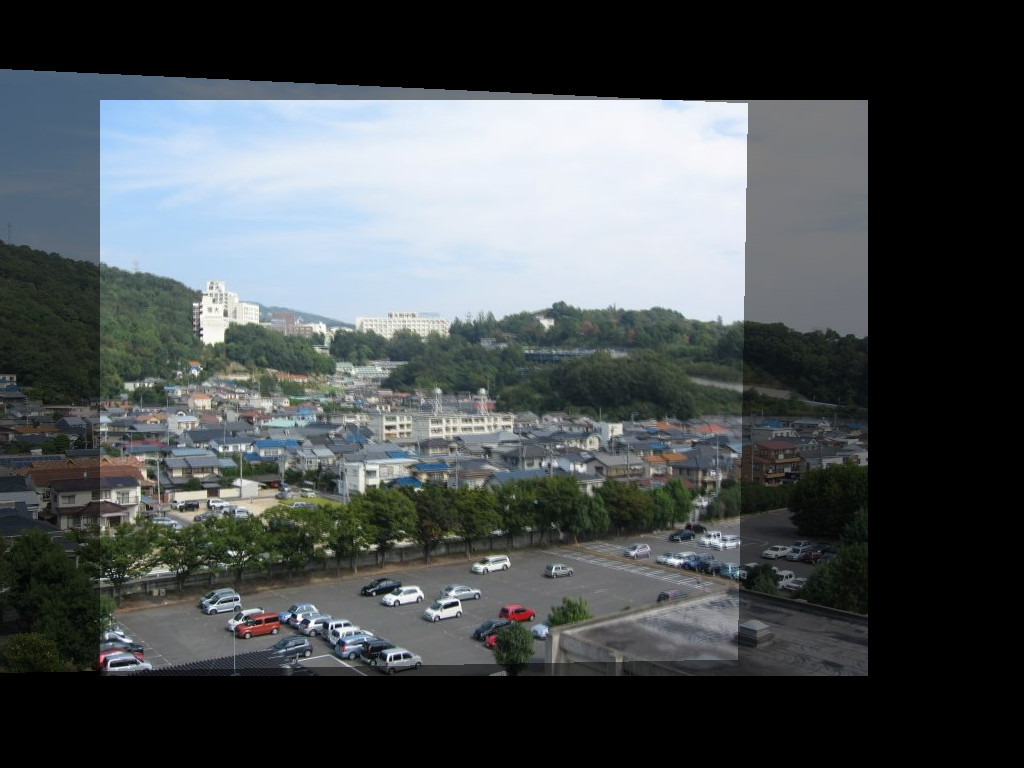
\includegraphics[scale=0.2]{3-1.W-12.jpg}
   \caption{特徴点12個の合成画像}
   \label{fig:3-1.W-12.jpg}
 \end{subfigure}
 \caption{特徴点数による合成画像の比較}
 \label{fig:comparison_W}
\end{figure}




\subsubsection{5組以上の特徴点を使った合成画像}
図\ref{fig:3-1.W-8.jpg}が特徴点の個数が8個の合成画像であり,図\ref{fig:3-1.W-12.jpg}が特徴点の個数が12個の合成画像である.
以下に画像合成に使用した w を載せる.このwの内,上から4行が特徴点4個,8行が特徴点8個,12行が特徴点12個の場合である.

\begin{Verbatim}[numbers=left, xleftmargin=10mm, numbersep=6pt,
                    fontsize=\small, baselinestretch=0.8]
  w=np.array([
44,42,165,65,
627,17,746,15,
58,558,183,563,
625,538,754,554,
113,187,233,202,
462,208,577,215,
162,523,281,533,
458,471,577,483,
269,285,387,294,
387,292,502,300,
288,350,404,362,
396,369,513,379,
]).reshape(-1,4)
\end{Verbatim}

特徴点は,4個のとき(図\ref{fig:3-1.W-4.jpg})が最も離れた4つの角で,8個のとき(図\ref{fig:3-1.W-8.jpg})では真ん中と端の中間あたりで,
12個のとき(図\ref{fig:3-1.W-12.jpg})では真ん中あたりに追加した.
画像を比較すると,特徴点の個数が多いほど綺麗に合成されていることが分かる.

\subsubsection{(u,v)の座標を自動修正する方法}
\begin{Verbatim}[numbers=left, xleftmargin=10mm, numbersep=6pt,
                    fontsize=\small, baselinestretch=0.8]
def sumOfSquaredDifference(w, im0, im1):
  for i in range(w.shape[0]):
    W=7
    x,y,u,v=w[i]

    tpl=im0[y-W:y+W+1,
            x-W:x+W+1]
    tgt=im1[v-W:v+W+1,
            u-W:u+W+1]
    res=np.zeros((7,7))
    for dv in range(-3,4):
      for du in range(-3,4):
        tgt=im1[v+dv-W:v+dv+W+1,
                u+du-W:u+du+W+1]
        res[dv+3,du+3]=((tpl-tgt)**2).sum()
    pos = np.array(np.unravel_index(np.argmin(res), res.shape))
    print(f"{i}[v,u] = {pos - [3,3]}")
\end{Verbatim}
上記のコードは,特徴点の周囲7x7ピクセルを比較して,最も差分が小さくなる(u,v)を探索するものである.
特徴点の周囲Wピクセルを切り出し,その中で(u,v)を中心に-3から+3までずらしたときの差分を計算し,最も差分が小さくなる(u,v)を選択している.
この方法により,手動で指定した特徴点の(u,v)座標を修正することができる.
しかしこのコードでは差分を計算するのみで,実際にwの(u,v)を更新する部分は含まれていないため,一度実行したのちに手動で更新する必要がある.

実行前のwは以下の通りである.
\begin{Verbatim}[numbers=left, xleftmargin=10mm, numbersep=6pt,
                    fontsize=\small, baselinestretch=0.8]
  w=np.array([
44,42,165,65,
627,17,746,15,
58,558,183,563,
625,538,754,554,
113,187,233,202,
462,208,577,215,
162,523,281,533,
458,471,577,483,
269,285,387,294,
387,292,502,300,
288,350,404,362,
396,369,513,379,
]).reshape(-1,4)
\end{Verbatim}
実行した出力は以下の通りである.
\begin{Verbatim}[numbers=left, xleftmargin=10mm, numbersep=6pt,
                    fontsize=\small, baselinestretch=0.8]
0[v,u] = [3 3]
1[v,u] = [-3 -2]
2[v,u] = [1 0]
3[v,u] = [2 1]
4[v,u] = [ 1 -1]
5[v,u] = [1 1]
6[v,u] = [-1  0]
7[v,u] = [1 0]
8[v,u] = [ 3 -2]
9[v,u] = [2 1]
10[v,u] = [-1  0]
11[v,u] = [1 0]
\end{Verbatim}
これを参考にして,wの(u,v)を修正すると以下のようになる

\begin{Verbatim}[numbers=left, xleftmargin=10mm, numbersep=6pt,
                    fontsize=\small, baselinestretch=0.8]
  w=np.array([
44,42,165,65,
627,17,746,15,
58,558,183,564,
625,538,755,556,
113,187,232,203,
462,208,578,216,
162,523,281,532,
458,471,577,484,
269,285,385,297,
387,292,503,302,
288,350,404,361,
396,369,513,380,
]).reshape(-1,4)
\end{Verbatim}

図\ref{fig:3.2-before.jpg},\ref{fig:3.2-after.jpg}が修正前と後の合成画像である.
\begin{figure}[h]
 \centering
 \begin{subfigure}[b]{0.45\textwidth}
   \centering
   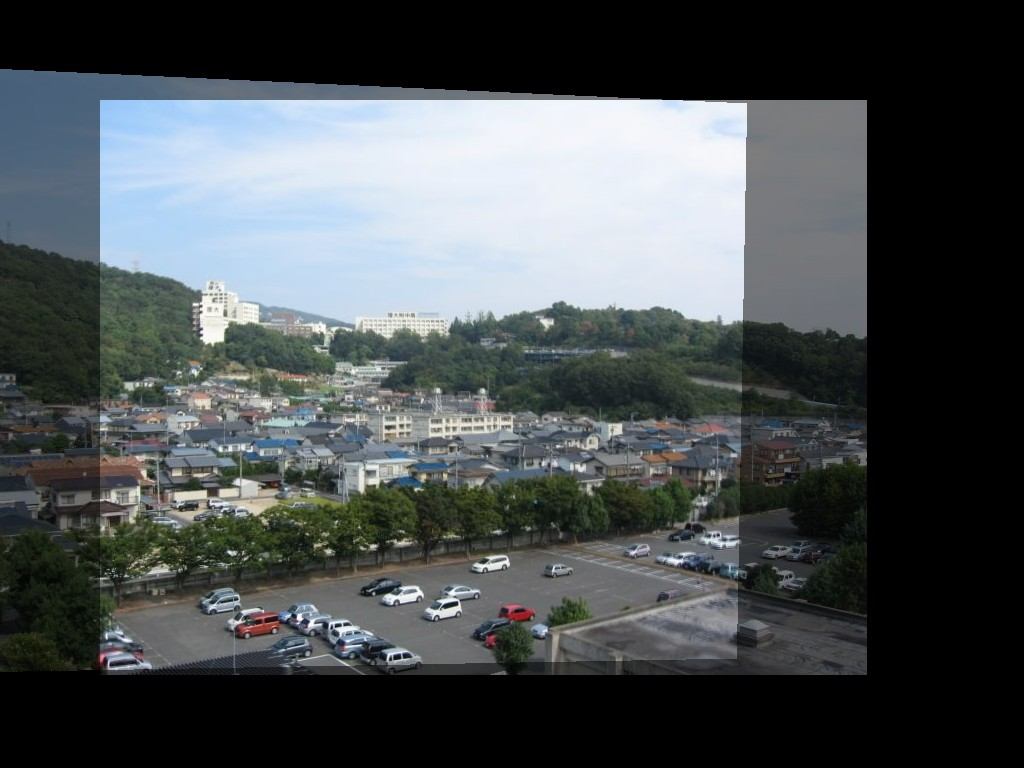
\includegraphics[scale=0.2]{3.2-before.jpg}
   \caption{自動修正前}
   \label{fig:3.2-before.jpg}
 \end{subfigure}
 \hspace{5mm}
 \begin{subfigure}[b]{0.45\textwidth}
   \centering
   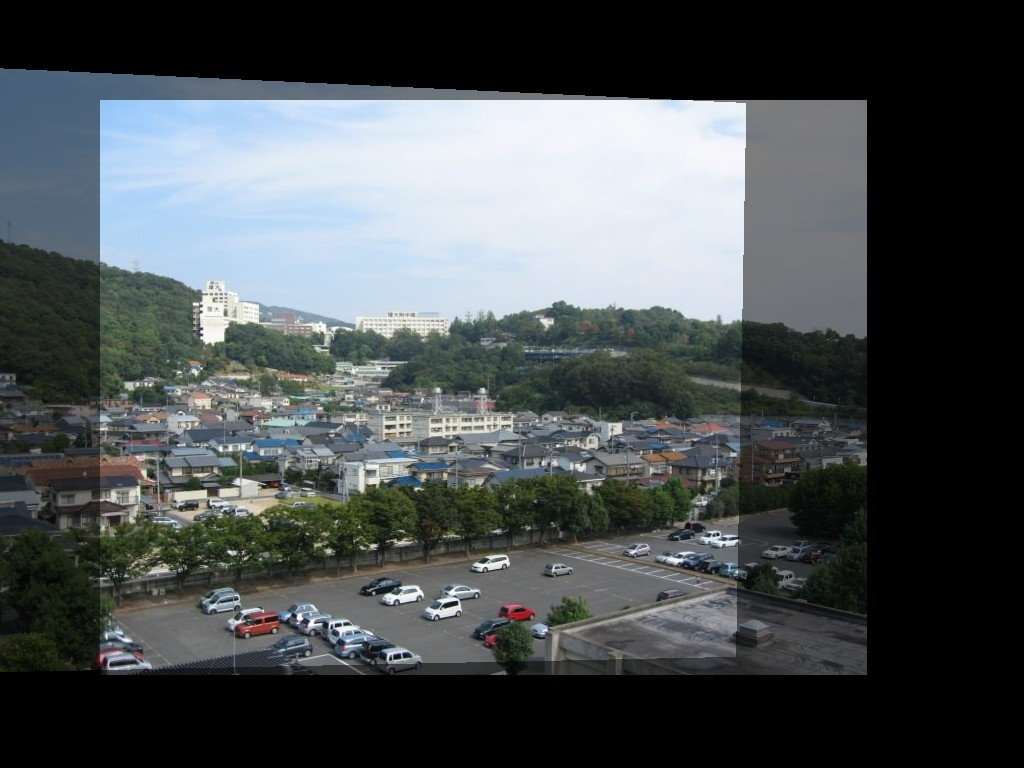
\includegraphics[scale=0.2]{3.2-after.jpg}
   \caption{自動修正後}
   \label{fig:3.2-after.jpg}
 \end{subfigure}
 \caption{自動修正前後の比較}
 \label{fig:comparison}
\end{figure}


これらの画像を比較すると,特に理科大の建物の文字の部分で修正前よりも綺麗に合成されていることが伺える.


\subsubsection{撮影した画像の合成}
使用する画像は図\ref{fig:IMG_5564.jpg},\ref{fig:IMG_5565.jpg}である.
\begin{figure}[h]
  \centering
  \begin{subfigure}[b]{0.3\textwidth}
    \centering
    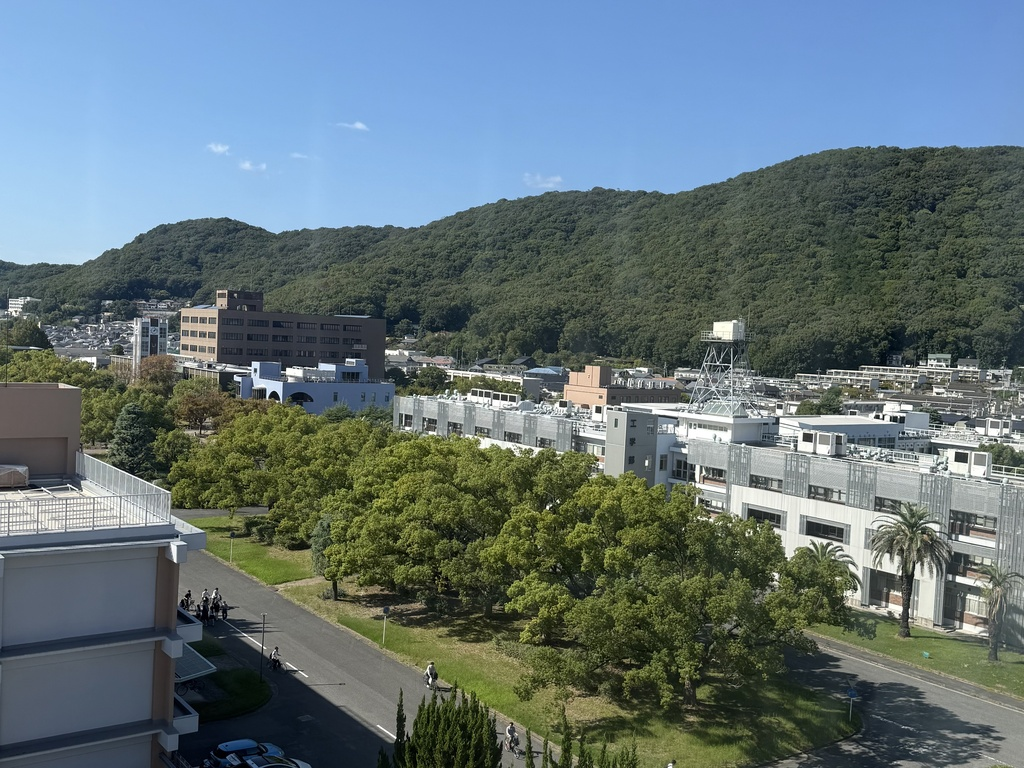
\includegraphics[width=\textwidth]{IMG_5564.jpg}
    \caption{撮影画像1}
    \label{fig:IMG_5564.jpg}
  \end{subfigure}
  \hfill
  \begin{subfigure}[b]{0.3\textwidth}
    \centering
    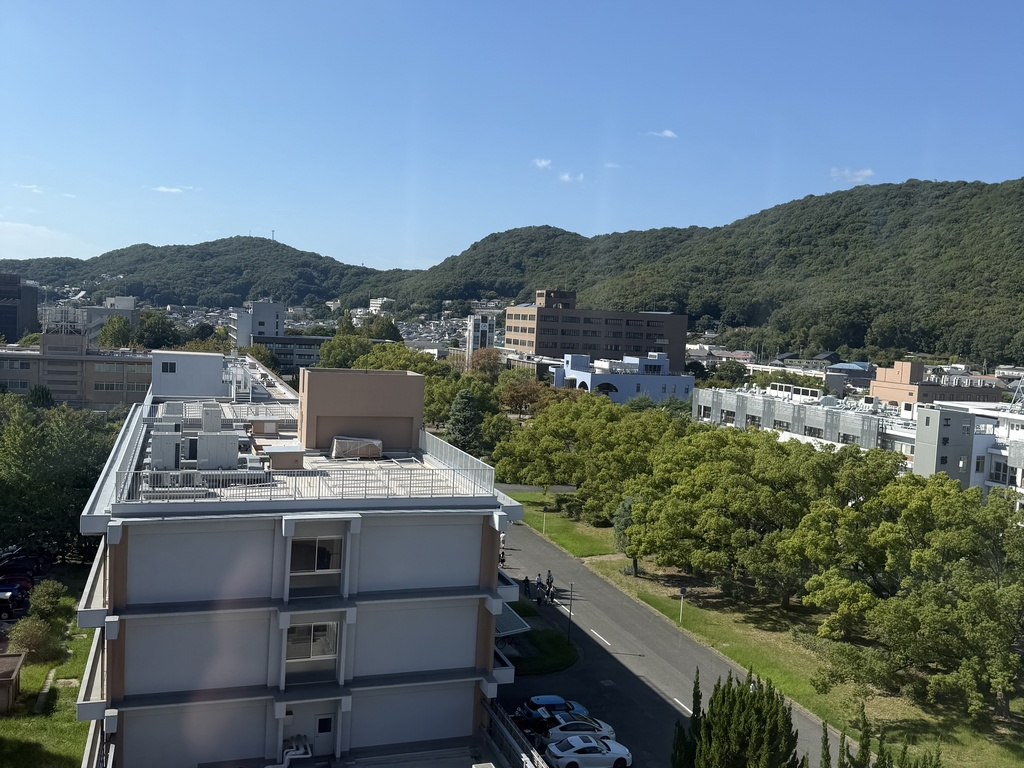
\includegraphics[width=\textwidth]{IMG_5565.jpg}
    \caption{撮影画像2}
    \label{fig:IMG_5565.jpg}
  \end{subfigure}
  \hfill
  \begin{subfigure}[b]{0.3\textwidth}
    \centering
    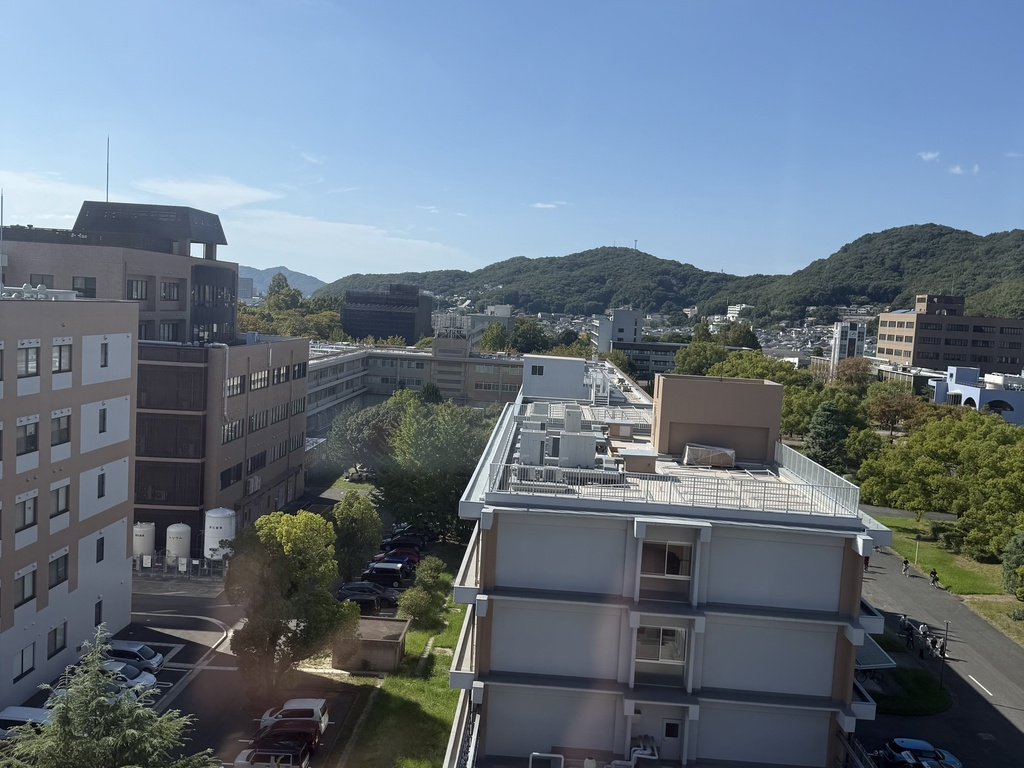
\includegraphics[width=\textwidth]{IMG_5566.jpg}
    \caption{撮影画像3}
    \label{fig:IMG_5566.jpg}
  \end{subfigure}
  \caption{3枚の撮影画像の比較}
  \label{fig:photo_comparison}
\end{figure}

使用する特徴点 w は以下の通りである((u, v)の自動修正済み).
\begin{Verbatim}[numbers=left, xleftmargin=10mm, numbersep=6pt,
                    fontsize=\small, baselinestretch=0.8]
  w=np.array([
909,362,598,366,
854,738,556,743,
500,519,178,549,
377,303,19,303,
]).reshape(-1,4)
\end{Verbatim}

そして,得られた合成画像が図\ref{fig:3.2-mypicture.jpg}である.
\begin{figure}[h]
 \centering
 \begin{subfigure}[b]{0.45\textwidth}
   \centering
   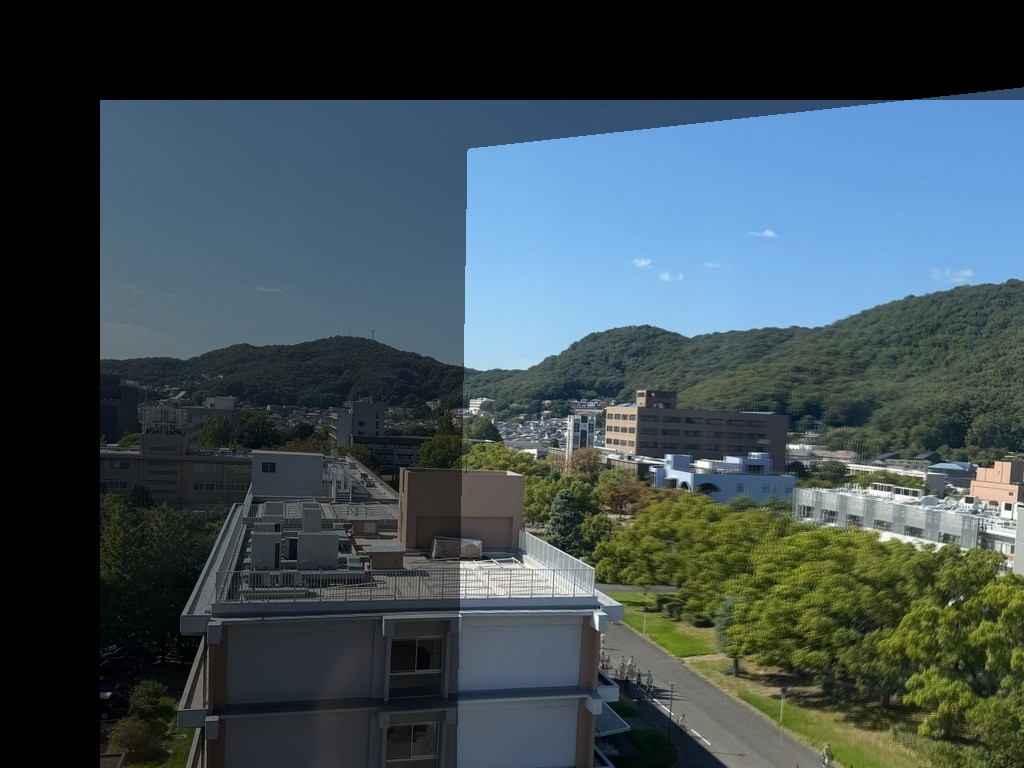
\includegraphics[scale=0.2]{3.2-mypicture.jpg}
   \caption{撮影画像の合成結果}
   \label{fig:3.2-mypicture.jpg}
 \end{subfigure}
 \hspace{5mm}
 \begin{subfigure}[b]{0.45\textwidth}
   \centering
   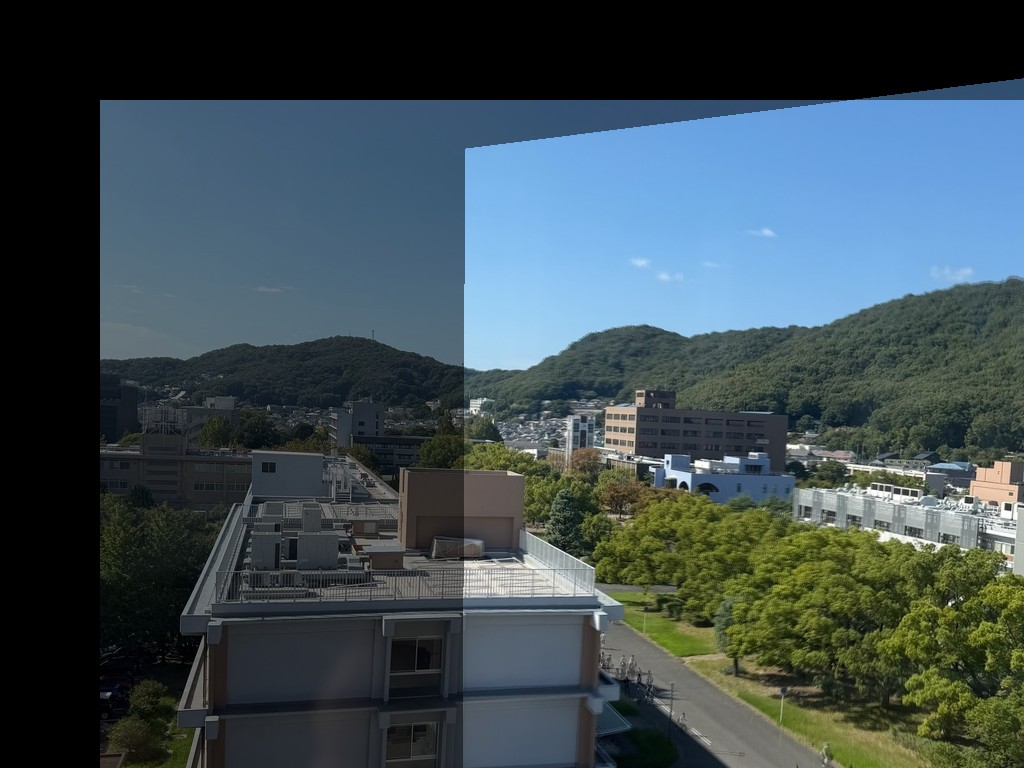
\includegraphics[scale=0.2]{3.2-mypicture_w-12.jpg}
   \caption{撮影画像の合成結果(特徴点12個)}
   \label{fig:3.2-mypicture_w-12.jpg}
 \end{subfigure}
 \caption{特徴点数による撮影画像の合成結果比較}
 \label{fig:comparison_mypicture}
\end{figure}


特徴点の個数を12個に増やした合成画像が図\ref{fig:3.2-mypicture_w-12.jpg}である.


\subsubsection{重なりの少ない画像の合成}
図\ref{fig:IMG_5564.jpg},\ref{fig:IMG_5565.jpg},\ref{fig:IMG_5566.jpg}の3枚の画像を使用し,
図\ref{fig:IMG_5564.jpg}と図\ref{fig:IMG_5566.jpg}を合成した.


使用した特徴点 w は以下の通りである.ただし,w1が図\ref{fig:IMG_5564.jpg}と図\ref{fig:IMG_5565.jpg}の特徴点,
w2が図\ref{fig:IMG_5565.jpg}と図\ref{fig:IMG_5566.jpg}の特徴点である.
\begin{Verbatim}[numbers=left, xleftmargin=10mm, numbersep=6pt,
                    fontsize=\small, baselinestretch=0.8]
  w1=np.array([
598,366,909,362,
556,743,854,738,
178,549,500,519,
19,303,377,303,
618,424,929,422,
366,364,668,358,
596,409,905,406,
553,503,856,500,
154,330,484,326,
253,370,565,362,
97,361,438,352,
97,323,438,319,
]).reshape(-1,4)

  w2=np.array([
83,699,455,668,
83,608,458,585,
85,513,463,499,
19,368,415,368,
569,360,953,372,
541,290,923,295,
376,299,734,306,
166,368,535,371,
580,563,960,601,
598,638,979,687,
589,239,983,237,
273,234,635,243,
]).reshape(-1,4)
\end{Verbatim}

得られた合成画像が図\ref{fig:3.2-mypicture-m2d.jpg}である.

また,3枚間の画像の合成結果は図\ref{fig:3.2-mypicture-m1dm2d.jpg}のようである.

\begin{figure}[h]
 \centering
 \begin{subfigure}[b]{0.45\textwidth}
   \centering
   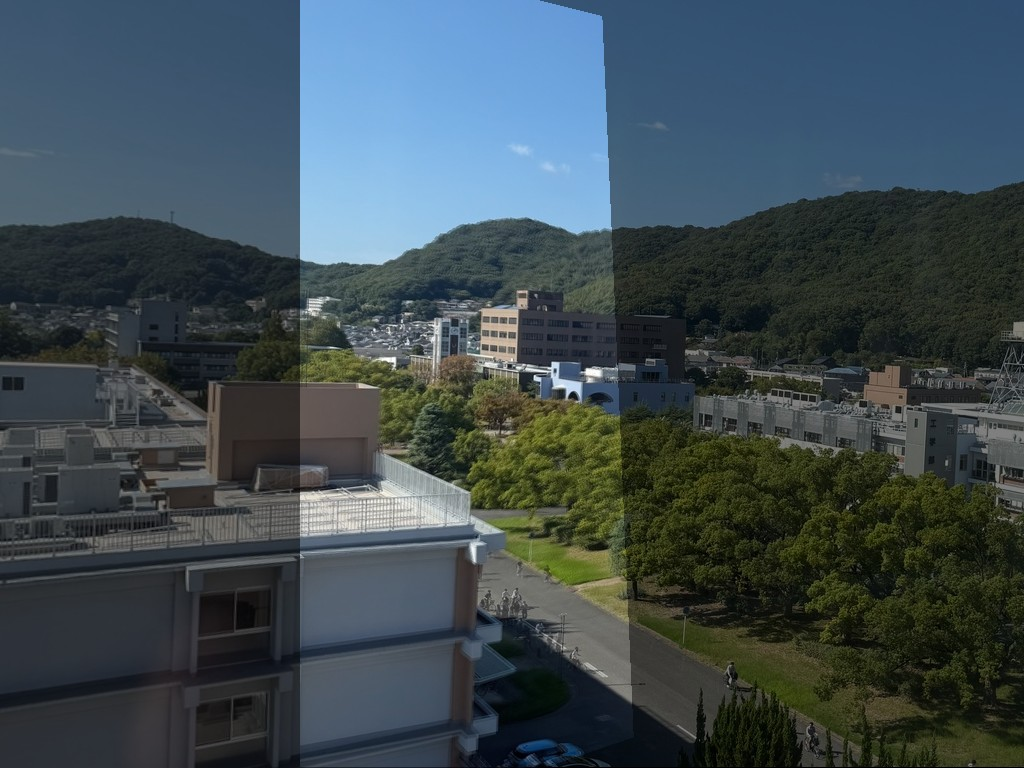
\includegraphics[scale=0.2]{3.2-mypicture-m2d.jpg}
   \caption{重なりの少ない画像の合成結果}
   \label{fig:3.2-mypicture-m2d.jpg}
 \end{subfigure}
 \hspace{5mm}
 \begin{subfigure}[b]{0.45\textwidth}
   \centering
   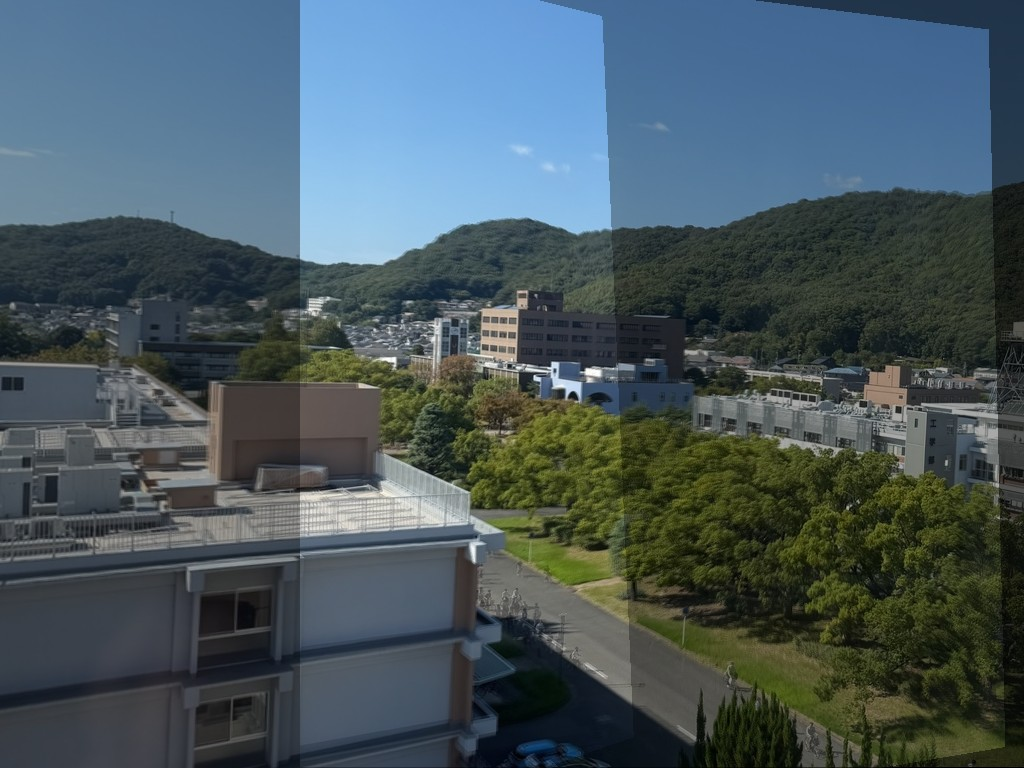
\includegraphics[scale=0.2]{3.2-mypicture-m1dm2d.jpg}
   \caption{3枚間の画像の合成結果}
   \label{fig:3.2-mypicture-m1dm2d.jpg}
 \end{subfigure}
 \caption{異なる重なり条件における画像合成結果の比較}
 \label{fig:comparison_m1dm2d}
\end{figure}






%--------------------------------------------------------------------%
\section{感想}

%--------------------------------------------------------------------%
% 参考文献
%   以下は,書き方の例である.実際に,参考にした書籍等を見て書くこと.
%   本文で引用する際は,\cite{book:algodata}などとすればよい.
%\begin{thebibliography}{99}
%  \bibitem{book:algodata} 平田富雄,アルゴリズムとデータ構造,森北出版,1990.
%  \bibitem{book:label2} 著者名,書名,出版社,発行年.
%  \bibitem{www:label3} WWWページタイトル,\spverb!https://example.of.too.long.url.jp/you.must.use.spverb/and.insert. a.space.somewhere.to.avoid.overfull.html!,アクセス日.
%\end{thebibliography}

%--------------------------------------------------------------------%
\end{document}
